\chapter{รายละเอียดของงานที่ปฏิบัติ}
\label{chapter:related-theory}

ผู้ช่วยผู้ให้คำปรึกษาด้านความปลอดภัย (Associate Security Consultant) ทำหน้าที่ค้นหาช่องโหว่และทดสอบเจาะระบบในระบบสารสนเทศของลูกค้า และรายงานช่องโหว่กลับไปยังลูกค้าเพื่อให้ลูกค้าแก้ไข พร้อมทั้งประเมินความยากง่ายในการเจาะระบบ ความร้ายแรงที่จะเกิดขึ้นหากเกิดการเจาะระบบ และคำแนะนำในการแก้ไขช่องโหว่

ในบทนี้จะกล่าวถึงขึ้นตอนวิธีการเจาะระบบก่อน จากนั้นจะพูดถึงพื้นฐานของเว็บแอปพลิเคชัน ที่สามารถนำไปประยุกต์ใช้ในการเจาะระบบได้ ท้ายที่สุดจะพูดถึงเครื่องมือที่ช่วยอำนวยความสะดวกในการเจาะระบบ พร้อมทั้งสาธิตวิธีการเจาะระบบบนระบบเว็บแอปพลิเคชันจำลองที่มีช่องโหว่

\section{การทดสอบเจาะระบบ (Penetration Testing)}

ก่อนที่จะกล่าวถึงขึ้นตอนวิธีการค้นหาช่องโหว่ในระบบ ควรเข้าใจถึงคำว่าช่องโหว่ก่อน คำว่า “ช่องโหว่” (Vulnerability) นั้นหมายถึงข้อผิดพลาดของซอฟต์แวร์ (Bug) ที่สามารถใช้ในทางที่ไม่เหมาะสมเพื่อหลบหลีกระบบความปลอดภัยที่ใช้งานอยู่ขณะนั้น โดยที่วิธีการใช้งานช่องโหว่เพื่อเข้าถึงข้อมูลที่ไม่สมควรที่จะเข้าถึงได้ ในวงการ Cyber Security เรียกว่าการ “Exploit” หรือ “เจาะระบบ” นั่นเอง \cite{what-is-an-exploit} ซึ่งช่องโหว่ใด ๆ สามารถมีวิธีการเจาะระบบได้หลากหลายวิธี

ยกตัวอย่างเช่น ซอฟต์แวร์ของของลูกค้าอาจมีข้อผิดพลาดที่ทำให้อุปกรณ์มีปัญหาเมื่อมีการทำการใส่ข้อมูลนำเข้าประหลาด การอัพโหลดไฟล์รูปภาพที่ไม่ได้มีการตรวจสอบข้อมูลที่อยู่ในไฟล์รูป เพื่อยืนยันว่าเป็นไฟล์รูปจริง ๆ จึงทำให้สามารถแทรกโค้ดที่อันตรายไปในรูป แล้วสามารถส่งคำสั่งอันตรายขึ้นไปรันบนเครื่องได้ อาจจะทำให้มีผู้ที่ไม่หวังดีสามารถดึงข้อมูลที่เป็นความลับของลูกค้าออกไปได้ ซึ่งการที่ไม่มีการตรวจสอบชนิดของไฟล์นั้นคือช่องโหว่ที่ต้องแก้ไข (Vulnerability) ส่วนการแทรกโค้ดที่อันตรายไปในรูป แล้วสามารถส่งคำสั่งอันตรายขึ้นไปรันบนเครื่องลูกค้าได้ โดยที่ไม่ต้องยืนยันตัวตนนั้นคือวิธีการหลบหลีกระบบความปลอดภัยโดยใช้ข้อผิดพลาดของระบบ (Exploit)

เมื่อค้นพบช่องโหว่แล้ว ควรจะเจาะระบบเพื่อยืนยันว่าในระบบของลูกค้านั้นมีช่องโหว่นั้นอยู่จริง ๆ จากนั้นจึงรายงานการมีอยู่ของช่องโหว่ วิธีการเจาะระบบ และคำแนะนำในการแก้ไขให้แก่ลูกค้า ซึ่งกระบวนการเหล่านี้เรียกว่า “Penetration Testing” หรือเรียกสั้น ๆ ว่า “Pentest” ซึ่งบุคคลที่เจาะระบบเรียกว่า “Pentester”

ขั้นตอนวิธีการทำ Penetration Testing มีขั้นตอนดังต่อไปนี้

\subsection{Pre-engagement}

ก่อนที่จะเริ่มการทำ Penetration Testing ผู้ทดสอบเจาะระบบต้องพูดคุยทำความเข้าใจกับลูกค้าให้เข้าใจในสิ่งที่ตรงกัน ความเข้าใจที่คลาดเคลื่อนอาจทำให้เกิดความเสียหายกับระบบของลูกค้าได้ เช่น หน้าที่ของผู้เขียนจะต้องทดสอบหาช่องโหว่ของระบบของลูกค้า ซึ่งจะตรงกับช่วง Testing ในวงจรการพัฒนาซอฟต์แวร์ ซึ่งไม่ได้มีแค่บริษัทของผู้เขียนที่ใช้งานตัวระบบของลูกค้า ณ ขณะนั้น อาจจะมีบริษัทอื่นเข้ามาทดสอบ Functional Test ของระบบก็เป็นได้ ซึ่งทางลูกค้าจะแยก Environment ของระบบไว้ให้ทั้งฝั่ง Pentester และ Functional Test หากมีการสื่อสารผิดพลาดเกิดขึ้น ทำให้เราทดสอบเจาะระบบบนฝั่ง Functional Test แล้วระบบเกิดล่มขึ้นมา จะทำให้การทำงานของฝั่ง Funtional Test ช้าลง และส่งผลเสียแก่ลูกค้า เป็นต้น
ในขั้นตอนนี้ผู้ทดสอบเจาะระบบควรใช้เวลาเข้าใจการเหตุผลว่าทำไมลูกค้าถึงอยากให้มีการทดสอบเจาะระบบ คำถามที่สำคัญที่ควรถามแก่ลูกค้าได้แก่ เพราะอะไรถึงอยากให้มีการเจาะระบบ สิ่งที่กลัวที่สุดหากถูกเจาะระบบจากผู้ที่ไม่หวังดีคืออะไร มีระบบหรืออุปกรณ์อะไรที่ควรระมัดระวังในการทดสอบเจาะระบบหรือไม่ (เช่น อุปกรณ์ทางการแพทย์ เป็นต้น)
นอกจากนี้ยังมีสิ่งที่สำคัญอื่น ๆ อีกที่ต้องตกลงกันกับลูกค้า เช่น

\begin{enumerate}
	\item Scope ตัวระบบที่จะให้ทดสอบอยู่บน IP อะไร สามารถใช้ช่องโหว่ที่ทำให้ตัวระบบล่มจนไม่สามารถใช้งานได้หรือไม่ 
	\item Testing Window ลูกค้าอาจจะต้องการให้ทดสอบเพี่ยงแค่ในวันที่หรือช่วงเวลาที่กำหนดให้เท่านั้น
	\item Contact Information ควรจะติดต่อใครหากเกิดสิ่งร้ายแรงขึ้น สามารถติด่อได้ 24 ชั่วโมงหรือไม่ ต้องใช้การเข้ารหัสจดหมายอิเล็กทรอนิกส์หรือไม่
	\item Documentation เอกสารสำคัญที่กำหนดสิทธ์ให้เราทำการทดสอบเจาะระบบ ยิ่งถ้าตัวระบบไม่ใช่ของลูกค้าโดยตรง แต่เป็นคู้ค้าของลูกค้าอีกทีนึง และควรจำกัดความรับผิดชอบหากมีอะไรร้ายแรงเกิดขึ้น
	\item Payment Terms การแบ่งจายเงิน ลูกค้าจะจ่ายเงินอย่างไร เมื่อไหร่ และเท่าไหร่
	\item Non-Disclosure Agreement สัญญาปกปิดข้อมูลของลูกค้า
\end{enumerate}

\subsection{Information Gathering}

ในขั้นตอนนี้ผู้ทดสอบเจาะระบบจะค้นคว้าหาข้อมูลภาพรวมของระบบว่ามีซอฟต์แวร์อะไรกำลังทำงานอยู่บ้าง เวอร์ชั่นอะไร แล้วแต่ละซอฟท์แวร์นั้นมีช่องโหว่ที่เคยเกิดขึ้นมาบ้างหรือไม่ กระบวนการนี้สามารถทำได้โดยการใช้เครื่องมือที่ช่วยในการทำ Port Scan\cite{???} เช่น Nmap\cite{???} เป็นต้น เมื่อตรวจพบเจอ Port\cite{???}  ที่ถูกเปิดใช้อยู่หมายเลข 80, 443 สามารถคาดเดาได้ว่าเป็นระบบ Web Application (เนื่องจากเปิด Port 80 และ 443) โดยที่เราสามารถตรวจสอบเวอร์ชั่นของ Web Server ได้โดยดูจาก HTTP Response Header เป็นต้น

\subsection{Threat Modeling}

อ้างอิงจากข้อมูลที่ได้จากขึ้นตอน Information Gathering มาลองคิดดูว่าหากมีผู้ทีไม่หวังดีต้อง
การจะเจาะระบบ จะมีเหตุการณ์ใดเกิดขึ้นบ้าง และทรัพยากรขององค์กรส่วนใดที่จะได้รับผลกระทบ เช่น ถ้าลูกค้าผลิตซอฟต์แวร์ของตัวเอง ผู้ไม่หวังดีก็อยากจะเข้าถึง Source Code ของระบบนั้น แล้วนำข้อมูลไปขายให้กับบริษัทคู่แข่งของลูกค้า เป็นต้น จากนั้นจึงสร้างแผนทดสอบการเจาะระบบ

\subsection{Vulnerability Analysis}

ขึ้นตอนนี้จะเริ่มการค้นหาช่องโหว่จากตัวระบบของลูกค้าโดยตรง โดยสามารถใช้เครื่องมือช่วยค้นหาช่องโหว่ได้ก็ดี หรือค้นหาช่องโหว่ด้วยมือก็ดี ซึ่งจะมีตัวอย่างในบทที่ 3 แต่ทว่าเครื่องมืออาจจะเกิดผลบวกเทียมได้ ดังนั้นต้องมีการตรวจสอบด้วยมือทุก ๆ ช่องโหว่ที่ถูกพบเจอด้วยเครื่องมืออีกครั้งหนึ่ง

นอกจากนี้ผู้ทดสอบเจาะระบบยังสามารถค้นหา Exploit สำหรับซอฟท์แวร์เวอร์ชั่นนั้น ๆ ได้ตามฐานข้อมูลสาธารณะเช่น www.exploit-db.com\cite{???}  หรือ Metasploit Framework\cite{???} เป็นต้น (บางเวอร์ชั่นอาจจะมีช่องโหว่ก็ได้ หรือไม่มีช่องโหว่ก็เป็นได้) ซึ่งผู้ทดสอบเจาะระบบจะต้องมั่นใจว่า Exploit ที่ใช้จะสามารถเจาะระบบได้จริง

\subsection{Exploitation}

ขั้นตอนนี้ผู้ทดสอบเจาะระบบเจาะช่องโหว่ที่พบเจอด้วย Exploit ของช่องโหว่นั้น ๆ ซึ่งถ้าหากเป็นช่องโหว่ที่เกิดจาก bussiness logic หรือ functional logic ผู้ทดสอบเจาะระบบต้องสร้าง Exploit ขึ้นมาเอง เช่น แอปของธนาคารที่ใช้โอนเงินสามารถโอนเงินที่มีจำนวนติดลบได้ ดั้งนั้น Exploit ของเราก็คือ จำนวนเงินที่มีค่าติดลบ เป็นต้น 

\subsection{Post Exploitation}

ในบางช่องโหว่เมื่อเจาะระบบแล้วอาจจะสามารถควบคุมเครื่องแม่ข่ายของลูกค้าได้ ซึ่งเราสามารถใช้เครื่องแม่ข่ายนี้เข้าถึงระบบภายใน (Internal)\cite{???}  ของลูกค้าต่อไป เพื่อเพิ่มระดับความรุนแรงของช่องโหว่ขึ้นได้ เช่น หากเราสามารถควบคุมเครื่อง Web Server ของลูกค้าได้ และเครื่องนั้นสามารถติดต่อกับระบบฐานข้อมูลลูกค้าภายใน เราสามารถใช้เครื่อง Web Server นั้นเป็นเครื่องตัวกลาง (Pivot)\cite{???} ในการเข้าถึงระบบฐานข้อมูลลูกค้าภายในได้ เป็นต้น

\subsection{Reporting}

ขั้นตอนสุดท้ายของการทำ Penetration Testing คือการเขียนรายงานส่งลูกค้า โดยจะรายงานช่องโหว่ที่พบเจอ (Findings) ความร้ายแรงของช่องโหว่นั้น ๆ และคำแนะนำในการแก้ไข
รายงานจะแบ่งออกเป็น 2 ประเภทดังนี้

\subsubsection{Executive Summary}

รายงานชนิดนี้อธิบายถึงเป้าหมายในการหาช่องโหว่ และอธิบายผลกระทบของช่องโหว่ในภาพรวม โดยรายงานชนิดนี้เขียนเพื่อให้ผู้บริหารที่ดูแลโครงการ หรือผู้ที่ไม่มีความรู้เฉพาะด้านอ่านเช่น จะไม่ใช้ประโยคว่า “ผู้เจาะระบบได้ใช้ช่องโหว่รหัส MS08-067 เพื่อให้ได้ Shell” แต่จะใช้ประโยคที่สื่อถึงผลกระทบของช่องโหว่แทน “ผู้เจาะระบบสามารถอ่านจดหมายอิเล็กทรอนิกส์ของทุกคนในองค์กรได้” เป็นต้น

\subsubsection{Technical Report}

รายงานชนิดนี้จะลงลึกถึงรายละเอียดด้านเทคนิค โดยจะมีรายละเอียดตั้งแต่การทำ Information Gathering ไปจนถึง Post Exploitation พร้อมทั้งประเมินความยากง่ายของการเจาะ และผลกระทบที่จะเกิดในแต่ละช่องโหว่ รายงานชนิดนี้ผู้ที่อ่านคือผู้พัฒนาระบบ


เนื่องจากลูกค้าของบริษัทที่ผู้เขียนได้ไปฝึกงานต้องการทราบเพียงช่องโหว่ที่มีอยู่ในระบบสารสนเทศเท่านั้น บริษัทที่ผู้เขียนไปฝึกงานจึงไม่ได้ทำตามขั้นตอนด้านบนทั้งหมด  แต่ทำเพียงแค่ขั้นตอน Pre-Engagement, Vunerability Analysis, Exploitation และ Reporting  ยกตัวอย่าง ลูกค้าธนาคารแห่งหนึ่งจะเปิดตัวแอปพลิเคชันใหม่บนมือถือ โดยตัวแอปพลิเคชั่นจะเชื่อมต่อกับ RESTful API ของธนาคาร ทางลูกค้าจึงจ้างบริษัทไปค้นหาเพียงแค่ช่องโหว่บนบนแอปพลิเคชั่นและ RESTful API เท่านั้น ไม่ได้อยากทราบว่าจะเกิดผลกระทบอะไรกับระบบสารสนเทศทั้งธนาคารหลังจากมีการทำ Exploit ของแต่ละช่องโหว่ จึงทำให้ไม่มีขั้นตอน Threat Modelling และ Post Exploitation

สุดท้ายลูกค้าจะให้ข้อมูลรายละเอียดเกี่ยวกับระบบมาในขั้นตอน Pre-Engagement จึงทำให้ไม่มีขั้นตอน Information Gathering

\section{พื้นฐานสำหรับการทำ Penetration Testing บนเว็บแอปพลิเคชัน}

การค้นหาช่องโหว่ในเว็บแอปพลิเคชันนั้น จะหาได้อย่างง่ายดายหากผู้ทดสอบเจาะระบบมีความรู้ด้านการพัฒนาเว็บแอปพลิเคชันนั้น หรือเคยพัฒนาเว็บแอปพลิเคชันนั้นมาก่อน ในหัวข้อนี้จะเขียนถึงสิ่งที่ควรรู้เป็นพื้นฐานในการทดสอบเจาะระบบเว็บแอปพลิเคชัน โดยผู้ทดสอบเจาะระบบควรมีพื้นฐานในการใช้ Command Line การเขียนภาษาโปรแกรม และพื้นฐานระบบเครือข่ายมาก่อนด้วย

\subsection{HTTP Protocol}

Hyper Text Transfer Protocol (HTTP) คือมาตราฐานการส่งข้อมูลสื่อสิ่งพิมพ์ (รวมถึง HTML) ผ่านอินเทอร์เน็ต ซึ่ง HTTP  ใช้สถาปัตยกรรมแบบ Client-Server \cite{https://developer.mozilla.org/en-US/docs/Web/HTTP/Overview} ซึ่ง Client จะเริ่มต้นติดต่อ Server ก่อนเพื่อร้องขอข้อมูลที่ต้องการ (Request) จากนั้นจะรอให้ฝั่ง Server ตอบกลับ เมื่อ Server ตอบกลับ (Response) Client จะนำข้อมูลไปใช้งานต่อไป ถ้าหากตัว Client เป็น Web Browser เช่น Chrome หรือ Firefox เป็นต้น Browser ก็จะนำ Response ที่เป็น HTML ไปแสดงผลบนหน้าจอผู้ใช้ต่อไป \cite{https://developer.mozilla.org/en-US/docs/Web/HTTP/Messages} 

โดยปกติ HTTP ส่งข้อมูลผ่านเครือข่ายในรูปแบบที่ไม่ได้เข้ารหัส หากมีผู้ที่ไม่ประสงค์ดีดักจับข้อมูลระหว่างทาง แล้วมีการส่งข้อมูลรหัสผ่านยืนยันตัวตน หรือรหัสบัตรเครดิต ผู้ประสงค์ร้ายสามารถนำข้อมูลที่ได้มาไปสร้างความเสียหายแก่เราได้ จึงมีการพัฒนา HTTP ที่มีการเข้ารหัสขึ้นมาที่เรียกว่า HTTPs เรามักจะเห็นรูปแม่กุญแจ หรือคำว่า SECURE ข้างซ้ายของแถบ URL ของเว็บที่ใช้ HTTPs เพื่อบ่งบอกถึงข้อมูลที่รับส่งจากเว็บไซต์นี้ผ่านการเข้ารหัส ถึงแม้ว่าจะมีใครมาดักจับข้อมูล ก็จะไม่สามารถอ่านได้ เพราะข้อมูลนั้นถูกเข้ารหัสไว้อยู่

\begin{figure}[!t]
	\centering
	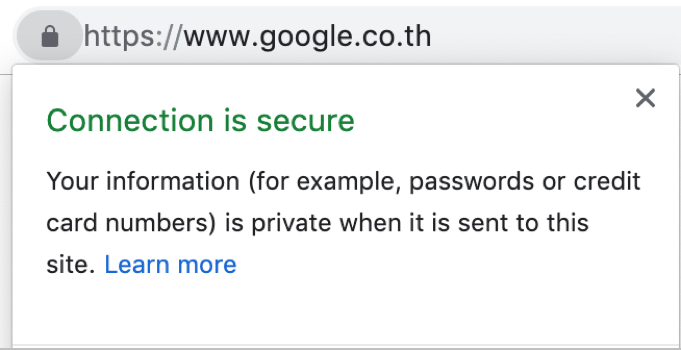
\includegraphics[width=0.6\columnwidth]{https.png}
	\caption{การเชื่อมต่อแบบ HTTPs บนเว็บไซต์ www.google.co.th}
	\label{Fig:https}
\end{figure}

\subsection{HTTP Cookie and Cookie Security}

เนื่องจาก HTTP เป็น Stateless Protocol ดังนั้น Server ไม่ทีทางรู้ได้ว่า แต่ละ Request ที่ส่งมานั้น มาจากผู้ใช้คนเดียวกันหรือไม่ ดังนั้นจึงมีสิ่งที่เรียกว่า Cookie เกิดขึ้น Cookie เป็น ข้อความรูปแบบ Key-Value ที่ Server ส่งให้กับ Client เพื่อที่ให้ Client แนบ Cookie นั้นมาทุก ๆ Request แล้ว Server จะได้รู้ว่าผู้ใช้คนใดเป็นคนส่งมา คล้าย ๆ กับการส่งจดหมายที่ต้องจ่าหน้าซองทุกครั้ง เพื่อที่จะได้รู้ว่าใครส่งมา \cite{https://developer.mozilla.org/en-US/docs/Web/HTTP/Cookies}

ในแต่ละ Domain จะมี Cookie แยกเป็นของตัวเอง และมีกฎในการอ่านเขียนดังนี้

\begin{enumerate}
	\item Cookie ที่ตั้งค่าโดย example.com สามารถถูกอ่านได้จากทุก ๆ Subdomain ของ example.com
	\item Cookie ที่ถูกเพิ่มโดย Subdomain สามารถอ่านได้โดย Subdomain นั้น และ Subdomain ของ Subdomain นั้น เช่น sub.example.com สามารถอ่าน Cookie ของ sub.example.com ได้ และ sub.example.com สามารถอ่าน Cookie ของ example.com ได้
	\item Subdomain สามารถตั้งค่า Cookie ของ Subdomain ของมันเอง และ Domain ที่เหนือกว่ามันได้ แต่ไม่สามารถตั้งค่า Cookie ของ Subdomain เครือญาติได้ เช่น foo.example.com ไม่สามารถ ตั้งค่า Cookie ของ bar.example.com ได้ แต่สามารถตั้งค่า Cookie ของ bar.foo.example.com และ example.com ได้
\end{enumerate}

นอกจากนี้ Server ควรตั้งค่า Secure Flag เพื่อให้ Cookie สามารถเข้าถึงผ่าน Https เท่านั้น และ HttpOnly Flag เพื่อไม่ให้ Javascript สามารถเข้าถึง Cookie ได้


